\section{Quitter le réseau}

Avec \SPRAY, les pairs peuvent quitter le réseau sans alerter qui que ce
soit. Nous ne faisons pas de distinctions particulières entre les départs et les
crashs. Toutefois, le protocole doit réagir à ces deux cas. En effet, sans
réactions, le réseau pourrait s'éffondrer pour cause de suppression d'arcs trop
zélé. Lorsqu'un pair rejoint le réseau, il y injecte $1+\ln(|\mathcal{N}|)$
arcs. Néanmoins, après plusieurs échanges, la vue partielle du pair rejoignant
le réseau est remplie par d'autres références. Ainsi, quand il quitte le réseau,
il entraine la suppression de $\ln(|\mathcal{N}|)$ arcs de sa vue partielle, et
$\ln(|\mathcal{N}|)$ arcs des pairs l'ayant dans leur vue partielle. Par
conséquent, sans moyens de gérer les départs, $2\ln(\mathcal{N}|)$ arcs sont
supprimés au lieu des $1+\ln(|\mathcal{N}|)$. Afin d'y remedier, chaque pair qui
détecte un crash peut rétablir une connexion avec l'un de ces voisins en
introduisant un doublon (doublon qui disparaitra rapidement après quelques
protocoles d'échange). La probabilité de réétablir une connexion est
$1-1\div{|\mathcal{P}|}$. Puisque ${|\mathcal{P}|}\approx \ln(|\mathcal{N}|)$
pairs ont detecté le crash dans leur vue partielle, il est probable qu'ils
recréent tous la connexion perdue, à l'exception d'un pair. De ce fait,
lorsqu'un pair quitte le réseau, il entraine la suppression d'un nombre d'arcs
correspondant approximativement au nombre d'arcs ajouté lors de la dernière
entrée de pair.

\begin{algorithm}[h]
  
\small
\algrenewcommand{\algorithmiccomment}[1]{\hskip2em$\rhd$ #1}

\newcommand{\comment}[1]{$\rhd$ #1}

\newcommand{\LINEFOR}[2]{%
  \algorithmicfor\ {#1}\ \algorithmicdo\ {#2} %
  }

\newcommand{\LINEIFTHEN}[2]{%
  \algorithmicif\ {#1}\ \algorithmicthen\ {#2} %
  }

\newcommand{\INDSTATE}[1][1]{\State\hspace{\algorithmicindent}}

\begin{algorithmic}[1]
  \Function{onPeerDown}{$q$} \hfill \comment{$q$: crashed/departed peer}  
  \State \textbf{let} $occ \leftarrow 0$;

  \For{\textbf{each} $\langle n,\,age\rangle \in \mathcal{P}$}
  \hfill \comment{remove and count}
  \If {($n=q$)}
  \State $\mathcal{P} \leftarrow \mathcal{P}\setminus \{\langle n,\,age\rangle \}$;
  \State $occ \leftarrow occ + 1$;
  \EndIf
  \EndFor

  \For{$i\leftarrow 0$ \textbf{to} $occ$} 
  \hfill \comment{probabilistically duplicates}
  \If{($rand()>{1\over{|\mathcal{P}|+occ}}$)}
  \State \textbf{let} $\langle n,\,\_ \,\rangle \leftarrow
  \mathcal{P}[\left\lfloor rand()*|\mathcal{P}|\right\rfloor]$;
  \State $\mathcal{P} \leftarrow \mathcal{P} \uplus
  \left\{\langle n,\, 0\rangle\right\}$;
  \EndIf
  \EndFor
  
  \EndFunction
  \Statex
  \Function{onArcDown}{$q,\,age$}
  \hfill \comment{$q$: arrival of the arc down}  
  \State $\mathcal{P} \leftarrow \mathcal{P}\setminus \{\langle q,\,age\rangle \}$;
  \State \textbf{let} $\langle n,\,\_ \,\rangle \leftarrow
  \mathcal{P}[\left\lfloor rand()*|\mathcal{P}|\right\rfloor]$;
  \State $\mathcal{P} \leftarrow \mathcal{P} \uplus
  \left\{\langle n,\, 0\rangle\right\}$;
  \hfill \comment{systematically duplicates}
  \EndFunction

\end{algorithmic}

  \caption{\label{net:algo:unreachable}The crash/departure handler of \SPRAY.}
\end{algorithm}

L'algorithme~\ref{net:algo:unreachable} montre la manière selon laquelle \SPRAY
gère les départs et crashs. La fonction $onPeerDown$ montre la réaction de
\SPRAY lorsque le pair $q$ est detecté comme parti ou défaillant. Dans un
premier temps, la fonction compte les occurences du pair $q$ dans la vue
partielle et les supprimes. Dans un second temps, une boucle ajoute de manière
probabiliste des doublons de références à des pairs déjà connus. La probabilité
dépend de la taille de la vue partielle avant la suppression.

\begin{figure*}
  \centering
  \subfloat[Figure A][Peer $p_1$ crashes.]{
    
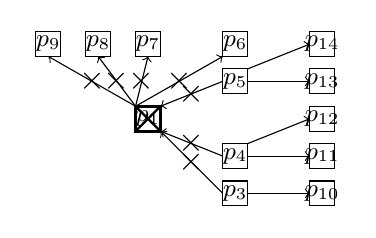
\begin{tikzpicture}[scale=0.9]

  \newcommand\X{35pt};
  \newcommand\Y{15pt};
  \large
  \draw[->](-5+\X, 1*\Y) --node{$\times$} ( 5pt,5pt);
  \draw[->](-5+\X, -1*\Y) --node{$\times$} ( 5pt,-5pt);
  \draw[->](-5+\X, -2*\Y) --node{$\times$} ( 5pt,-5pt);

  \draw[->](-5pt,5pt)--node{$\times$}(-10-2*\Y,-5+2*\Y); %% 1 -> 9
  \draw[->](-5pt,5pt)--node{$\times$}(-5-1*\Y,-5+2*\Y); %% 1 ->8 
  \draw[->](-5pt,5pt)--node{$\times$}(0pt,-5+2*\Y); %% 1 -> 7
  \draw[->](-5pt,5pt)--node{$\times$}(-5+\X,-5+2*\Y); %% 1 -> 6
  \normalsize
  \draw[->](5+ 1*\X, 5+ 1*\Y)--(-5+2*\X, 2*\Y); %% 5 -> 14
  \draw[->](5+1*\X,  1*\Y)--(-5+2*\X, 1*\Y); %% 5 -> 13 
  
  \draw[->](5+\X, 5-\Y) -- (-5+2*\X,0pt); %% 4 -> 12
  \draw[->](5+\X, -\Y) -- (-5+2*\X, -\Y); %% 4 -> 11
  
  \draw[->](5+\X, -2*\Y) -- (-5+2*\X, -2*\Y);
  
  \small
  \draw[fill=white,very thick]
  (0*\X, 0*\Y) node{$p_1$} +(-5pt,-5pt) rectangle +(5pt,5pt);
  \draw[thick] (-5pt,-5pt) -- (5pt,5pt);
  \draw[thick] (-5pt, 5pt) -- (5pt,-5pt);
  
  \draw[fill=white]
  (1*\X,1*\Y) node{$p_5$} +(-5pt,-5pt) rectangle +(5pt,5pt);
  \draw[fill=white]
  (1*\X,-1*\Y) node{$p_4$} +(-5pt,-5pt) rectangle +(5pt,5pt);
  \draw[fill=white]
  (1*\X,-2*\Y) node{$p_3$} +(-5pt,-5pt) rectangle +(5pt,5pt);

  \draw[fill=white](\X,2*\Y) node{$p_6$} +(-5pt,-5pt) rectangle +(5pt,5pt);

  \draw[fill=white]( 0*\X,2*\Y)
  node{$p_7$} +(-5pt,-5pt) rectangle +(5pt,5pt);
  \draw[fill=white](-5+-\Y,2*\Y)node{$p_8$} +(-5pt,-5pt) rectangle +(5pt,5pt);
  \draw[fill=white](-10+-2*\Y,2*\Y) node{$p_9$} +(-5pt,-5pt) rectangle +(5pt,5pt);
  
  \draw[fill=white](2*\X,2*\Y)node{$p_{14}$} +(-5pt,-5pt) rectangle +(5pt,5pt);
  \draw[fill=white](2*\X,1*\Y)node{$p_{13}$} +(-5pt,-5pt) rectangle +(5pt,5pt);
  \draw[fill=white](2*\X,0*\Y)node{$p_{12}$} +(-5pt,-5pt) rectangle +(5pt,5pt);
  \draw[fill=white](2*\X,-1*\Y)node{$p_{11}$}+(-5pt,-5pt) rectangle +(5pt,5pt);
  \draw[fill=white](2*\X,-2*\Y)node{$p_{10}$}+(-5pt,-5pt) rectangle +(5pt,5pt);

\end{tikzpicture}}
  \hspace{10pt}
  \subfloat[Figure B][The peers $p_{3-5}$ notice that they cannot
  reach $p_1$ anymore.]{
    
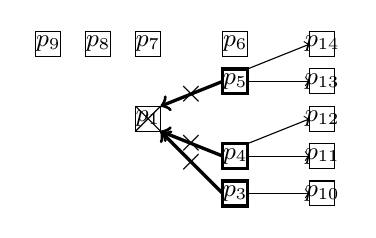
\begin{tikzpicture}[scale=0.9]

  \newcommand\X{35pt};
  \newcommand\Y{15pt};

  \large
  \draw[->, very thick](-5+\X, 1*\Y) -- node{$\times$} ( 5pt,5pt);
  \draw[->, very thick](-5+\X, -1*\Y) --node{$\times$} ( 5pt,-5pt);
  \draw[->, very thick](-5+\X, -2*\Y) --node{$\times$} ( 5pt,-5pt);

  \normalsize

  \draw[->](5+ 1*\X, 5+ 1*\Y)--(-5+2*\X, 2*\Y); %% 5 -> 14
  \draw[->](  5+1*\X, 1*\Y)--(-5+2*\X, 1*\Y); %% 5 -> 13 (v)
  
  \draw[->](5+\X, 5-\Y) -- (-5+2*\X,0pt); %% 4 -> 12
  \draw[->](5+\X, -\Y) -- (-5+2*\X, -\Y); %% 4 -> 11
  
  \draw[->](5+\X, -2*\Y) -- (-5+2*\X, -2*\Y);
  
  \small
  \draw[fill=white]
  (0*\X, 0*\Y) node{$p_1$} +(-5pt,-5pt) rectangle +(5pt,5pt);
  \draw (-5pt,-5pt) -- (5pt,5pt);
  \draw (-5pt, 5pt) -- (5pt,-5pt);
  
  \draw[fill=white, very thick]
  (1*\X,1*\Y) node{$p_5$} +(-5pt,-5pt) rectangle +(5pt,5pt);
  \draw[fill=white, very thick]
  (1*\X,-1*\Y) node{$p_4$} +(-5pt,-5pt) rectangle +(5pt,5pt);
  \draw[fill=white, very thick]
  (1*\X,-2*\Y) node{$p_3$} +(-5pt,-5pt) rectangle +(5pt,5pt);

  \draw[fill=white](\X,2*\Y) node{$p_6$} +(-5pt,-5pt) rectangle +(5pt,5pt);

  \draw[fill=white]( 0*\X,2*\Y)
  node{$p_7$} +(-5pt,-5pt) rectangle +(5pt,5pt);
  \draw[fill=white](-5+-\Y,2*\Y)node{$p_8$} +(-5pt,-5pt) rectangle +(5pt,5pt);
  \draw[fill=white](-10+-2*\Y,2*\Y) node{$p_9$} +(-5pt,-5pt) rectangle +(5pt,5pt);
  
  \draw[fill=white](2*\X,2*\Y)node{$p_{14}$} +(-5pt,-5pt) rectangle +(5pt,5pt);
  \draw[fill=white](2*\X,1*\Y)node{$p_{13}$} +(-5pt,-5pt) rectangle +(5pt,5pt);
  \draw[fill=white](2*\X,0*\Y)node{$p_{12}$} +(-5pt,-5pt) rectangle +(5pt,5pt);
  \draw[fill=white](2*\X,-1*\Y)node{$p_{11}$}+(-5pt,-5pt) rectangle +(5pt,5pt);
  \draw[fill=white](2*\X,-2*\Y)node{$p_{10}$}+(-5pt,-5pt) rectangle +(5pt,5pt);

\end{tikzpicture}}
  \hspace{10pt}
  \subfloat[Figure C][The peers $p_3$ and $p_5$ choose to establish
  a duplicate with one of their existing neighbor.]{
    
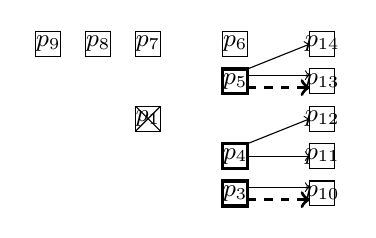
\begin{tikzpicture}[scale=0.9]

  \newcommand\X{35pt};
  \newcommand\Y{15pt};

  \draw[->](5+ 1*\X, 5+ 1*\Y)--(-5+2*\X, 2*\Y); %% 5 -> 14
  \draw[->](5+1*\X, 2.5+ 1*\Y)--(-5+2*\X, 2.5+ 1*\Y); %% 5 -> 13 (^)
  \draw[->,dashed, very thick]
  (  5+1*\X,-2.5+1*\Y)--(-5+2*\X,-2.5+1*\Y); %% 5 -> 13 (v)
  
  \draw[->](5+\X, 5-\Y) -- (-5+2*\X,0pt); %% 4 -> 12
  \draw[->](5+\X, -\Y) -- (-5+2*\X, -\Y); %% 4 -> 11
  
  \draw[->](5+\X, 2.5-2*\Y) -- (-5+2*\X, 2.5-2*\Y);
  \draw[->,dashed, very thick](5+\X, -2.5-2*\Y) -- (-5+2*\X , -2.5-2*\Y);
  
  \small
  \draw[fill=white]
  (0*\X, 0*\Y) node{$p_1$} +(-5pt,-5pt) rectangle +(5pt,5pt);
  \draw (-5pt,-5pt) -- (5pt,5pt);
  \draw (-5pt, 5pt) -- (5pt,-5pt);
  
  \draw[fill=white, very thick]
  (1*\X,1*\Y) node{$p_5$} +(-5pt,-5pt) rectangle +(5pt,5pt);
  \draw[fill=white, very thick]
  (1*\X,-1*\Y) node{$p_4$} +(-5pt,-5pt) rectangle +(5pt,5pt);
  \draw[fill=white, very thick]
  (1*\X,-2*\Y) node{$p_3$} +(-5pt,-5pt) rectangle +(5pt,5pt);

  \draw[fill=white](\X,2*\Y) node{$p_6$} +(-5pt,-5pt) rectangle +(5pt,5pt);

  \draw[fill=white]( 0*\X,2*\Y)
  node{$p_7$} +(-5pt,-5pt) rectangle +(5pt,5pt);
  \draw[fill=white](-5+-\Y,2*\Y)node{$p_8$} +(-5pt,-5pt) rectangle +(5pt,5pt);
  \draw[fill=white](-10+-2*\Y,2*\Y) node{$p_9$} +(-5pt,-5pt) rectangle +(5pt,5pt);
  
  \draw[fill=white](2*\X,2*\Y)node{$p_{14}$} +(-5pt,-5pt) rectangle +(5pt,5pt);
  \draw[fill=white](2*\X,1*\Y)node{$p_{13}$} +(-5pt,-5pt) rectangle +(5pt,5pt);
  \draw[fill=white](2*\X,0*\Y)node{$p_{12}$} +(-5pt,-5pt) rectangle +(5pt,5pt);
  \draw[fill=white](2*\X,-1*\Y)node{$p_{11}$}+(-5pt,-5pt) rectangle +(5pt,5pt);
  \draw[fill=white](2*\X,-2*\Y)node{$p_{10}$}+(-5pt,-5pt) rectangle +(5pt,5pt);

\end{tikzpicture}}
  \caption{\label{net:fig:crashexample}Example of \SPRAY's crash/leaving
    handler. }
\end{figure*}

La figure~\ref{net:fig:crashexample} montre le fonctionnement de la gestion des
pairs detecté comme étant parti ou défaillant. Le pair $p_1$ quitte le réseau
sans en informer le réseau. Avec lui, $7$ connexions sont inutilisables. Les
pairs $p_3$, $p_4$, et $p_5$ ont toujours une référence vers $p_1$ dans leur vue
partielle. Le pair $p_5$ a $1-{1\div{|\mathcal{P}_5|}}={2\div{3}}$ chances de
remplacer la connexion. Dans ce cas, il double la référence à $p_{13}$. De la
même manière, $p_3$ et $p_4$ détectent $p_1$ comme étant injoignable et agissent
en conséquence. Seul $p_3$ crée un doublon remplaçant. Au total, $5$ connexions
ont été supprimées.

L'exemple montre que certains des pairs ont rétabli une connexion lorsqu'ils ont
détécté qu'un pair était injoignable. La probabilité dépend de la vue partielle
de chacun de ces pairs. En moyenne, l'un de ces pairs va vraisemblablement
supprimer l'arc inutilisable alors que les autres vont simplement le
remplacer. Dans l'exemple, le pair $p_1$ a injecté $5$ arcs lors de son entrée
dans le réseau. $7-2 = 5$ arcs ont été supprimés lors de son départ. Le nombre
global d'arcs dans le réseau reste d'ordre logarithmique comparé à la taille du
réseau. Toutefois, nous remarquons que la connectivité n'est pas entièrement
garantie (seulement avec la forte probabilité impliquée par les graphes
aléatoires). En effet, si le pair $p_1$ est le seul pont entre deux groupes de
pairs, ajouter des arcs n'est pas suffisant pour garantir la connectivité.

L'algorithme~\ref{net:algo:unreachable} montre aussi que \SPRAY distingue les
pairs qui sont injoignables des arcs inutilisables. En effet, la fonction
$onArcDown$ gère les connexions dont la création a échoué. Ces arcs sont
systématiquement remplacés par un doublon. De ce fait, le nombre d'arc reste
bien constant. La distinction $onPeerDown$ avec $onArcDown$ est necessaire car
la première doit supprimer une petite quantité d'arcs. Sans cette suppression,
le nombre d'arcs augmenterait de manière incontrollée avec les entrées et
sorties de pairs.
